Ecco le function da noi utilizzate nel corso del capitolo :

\begin{itemize}

\item Formula dei trapezi composita :
\lstinputlisting[language=Matlab]{cap_5_6/trapeziComposita.m}

\item Formula dei trapezi adattiva :
\lstinputlisting[language=Matlab]{cap_5_6/trapeziAdattiva.m}

\item Formula di Simpson composita :
\lstinputlisting[language=Matlab]{cap_5_6/simpsonComposita.m}

\item Formula di Simpson adattiva
\lstinputlisting[language=Matlab]{cap_5_6/simpsonAdattiva.m}

\end{itemize}

\subsection{\textbf{Esercizio 5.1}}
\lstinputlisting[language=Matlab]{cap_5_6/es1/es1.m}
\subsection{\textbf{Esercizio 5.2}}
\lstinputlisting[language=Matlab]{cap_5_6/es2/es2.m}
\begin{figure}
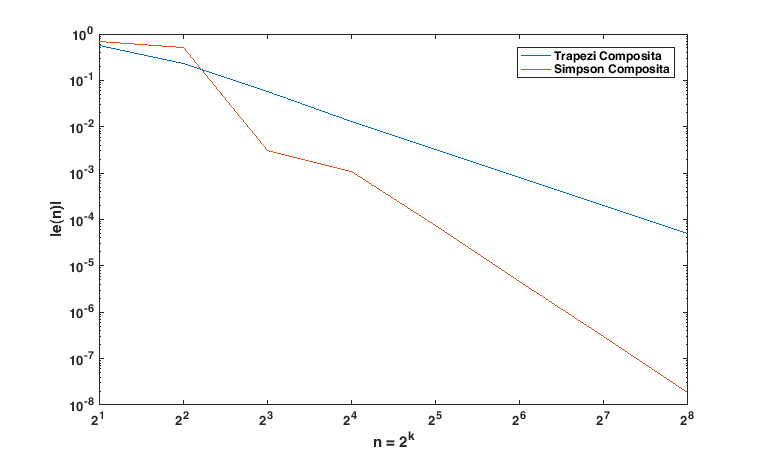
\includegraphics[width=\textwidth]{cap_5_6/es2/error.png}
\caption{Andamento dell'errore per i metodi di Quadratura}
\label{QuadrErr}
\end{figure}
\begin{figure}
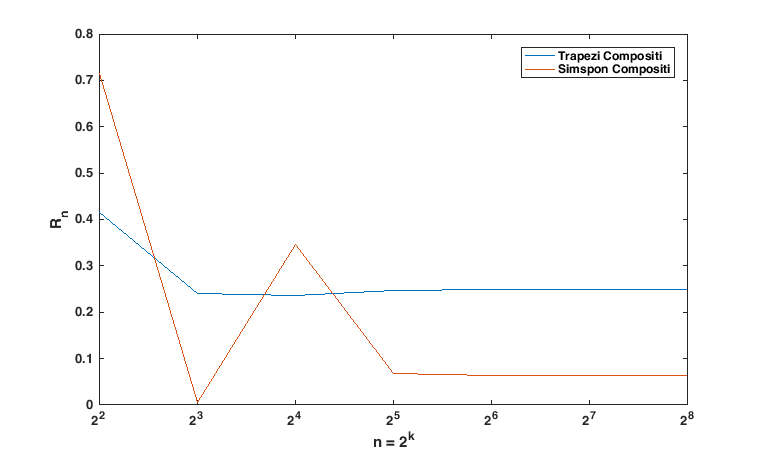
\includegraphics[width=\textwidth]{cap_5_6/es2/rapp_err.png}
\caption{Andamento del Rapporto tra gli errori per i metodi di Quadratura}
\label{QuadrRapp}
\end{figure}

\subsection{\textbf{Esercizio 5.3}}
\lstinputlisting[language=Matlab]{cap_5_6/es3/es3.m}
\subsection{\textbf{Esercizio 5.4}}
\lstinputlisting[language=Matlab]{cap_5_6/jacobi.m}
\lstinputlisting[language=Matlab]{cap_5_6/gaussSeidel.m}
\subsection{\textbf{Esercizio 5.5}}
\lstinputlisting[language=Matlab]{cap_5_6/es5/es5.m}

Il sistema $A = \left(\begin{array}{ccc} -4 & 2 & 1\\ 1 & 6 & 2\\ 1 & -2 & 5 \end{array}\right)$
\subsection{\textbf{Esercizio 5.6}}
\lstinputlisting[language=Matlab]{cap_5_6/es6/es6.m}
Nel grafico \ref{PR_comparison} \'e mostrato l'andamento dei vari metodi numerici per il calcolo dell'autovettore.
Si nota come al crescere della tolleranza i metodi di Jacobi e delle Potenze non divergano sostanzialmente, mentre il metodo di Gauss-Seidel mostra una maggior efficienza anche per valori di tolleranza ridotti.

